\ifx\allfiles\undefined
\documentclass[12pt, a4paper, oneside, UTF8]{ctexbook}
\def\path{../config}
\input{\path/package.tex}

% 定理环境设置
\input{\path/theorem1_zh.tex}

\input{\path/custom.tex}

% 修改参数改变封面样式，0 默认原始封面、内置其他1、2、3种封面样式
\def\myIndex{3}


\ifnum\myIndex>0
    \input{\path/cover_package_\myIndex} 
\fi

\def\myTitle{高等数学笔记}
\def\myAuthor{M.K.}
\def\myDateCover{\today}
\def\myDateForeword{\today}
\def\myForeword{前言}
\def\myForewordText{
    
    这是一个基于\LaTeX{}模板的高数笔记．
    内容参考了包括但不限于以下资料：
    \begin{itemize}
        \item 《高等数学》（同济大学出版社）第七版
        \item 《吉米多维奇高等数学习题精选精讲》（山东科学技术出版社）第二版
        \item 《高等数学作业集》（哈尔滨工业大学出版社）第一版
        \item \href{https://space.bilibili.com/1035929235}{B站UP主：一高数}的高数课程
        \item \href{https://space.bilibili.com/42428180}{B站UP主：考研竞赛数学}的试题讲解与高数课程
        \item \href{https://space.bilibili.com/391930545}{B站UP主：Maki的完美算数教室}的高数内容

    \end{itemize}

    封面来源于\href{https://www.pixiv.net/users/3952}{おにねこ}的作品\href{https://www.pixiv.net/artworks/136551599}{雨雫とプレアデス}
    如有侵权请联系我删除．
}
\def\mySubheading{副标题}


\begin{document}
% \input{../config/cover}
\else
\fi

\chapter{空间解析几何}

\section{空间中的直线和平面}

\subsection{直线、平面的相对位置关系}

\subsubsection{两平面的位置关系}
设平面 $\pi_1: A_1x+B_1y+C_1z+D_1=0$，法向量 $\boldsymbol{n_1}=(A_1, B_1, C_1)$；\\
平面 $\pi_2: A_2x+B_2y+C_2z+D_2=0$，法向量 $\boldsymbol{n_2}=(A_2, B_2, C_2)$．

\begin{itemize}
    \item \textbf{夹角}：两平面的夹角 $\theta$（二面角的锐角或直角）满足：
    \[ 
        \cos\theta = \frac{|\boldsymbol{n_1} \cdot \boldsymbol{n_2}|}{|\boldsymbol{n_1}||\boldsymbol{n_2}|} = \frac{|A_1A_2+B_1B_2+C_1C_2|}{\sqrt{A_1^2+B_1^2+C_1^2}\sqrt{A_2^2+B_2^2+C_2^2}} 
    \]
    \item \textbf{垂直}：$\pi_1 \perp \pi_2 \iff \boldsymbol{n_1} \cdot \boldsymbol{n_2} = 0 \iff A_1A_2+B_1B_2+C_1C_2=0$
    \item \textbf{平行}：$\pi_1 \parallel \pi_2 \iff \boldsymbol{n_1} \parallel \boldsymbol{n_2} \iff \dfrac{A_1}{A_2}=\dfrac{B_1}{B_2}=\dfrac{C_1}{C_2}$
\end{itemize}

\subsubsection{两直线的位置关系}
设直线 $L_1$ 的方向向量为 $\boldsymbol{s_1}=(m_1, n_1, p_1)$，直线 $L_2$ 的方向向量为 $\boldsymbol{s_2}=(m_2, n_2, p_2)$．

\begin{itemize}
    \item \textbf{夹角}：两直线的夹角 $\varphi$ ($0 \le \varphi \le \frac{\pi}{2}$) 满足：
    \[ 
        \cos\varphi = \frac{|\boldsymbol{s_1} \cdot \boldsymbol{s_2}|}{|\boldsymbol{s_1}||\boldsymbol{s_2}|} 
    \]
    \item \textbf{垂直}：$L_1 \perp L_2 \iff \boldsymbol{s_1} \cdot \boldsymbol{s_2} = 0 \iff m_1m_2+n_1n_2+p_1p_2=0$
    \item \textbf{平行}：$L_1 \parallel L_2 \iff \boldsymbol{s_1} \parallel \boldsymbol{s_2} \iff \dfrac{m_1}{m_2}=\dfrac{n_1}{n_2}=\dfrac{p_1}{p_2}$
\end{itemize}

\subsubsection{直线与平面的位置关系}
设直线 $L$ 的方向向量为 $\boldsymbol{s}=(m, n, p)$，平面 $\pi$ 的法向量为 $\boldsymbol{n}=(A, B, C)$．

\begin{itemize}
    \item \textbf{夹角}：直线与平面的夹角 $\psi$ ($0 \le \psi \le \frac{\pi}{2}$) 满足：
    \[ 
        \sin\psi = \frac{|\boldsymbol{s} \cdot \boldsymbol{n}|}{|\boldsymbol{s}||\boldsymbol{n}|} 
    \]
    \item \textbf{垂直}：$L \perp \pi \iff \boldsymbol{s} \parallel \boldsymbol{n} \iff \dfrac{m}{A}=\dfrac{n}{B}=\dfrac{p}{C}$
    \item \textbf{平行}：$L \parallel \pi \iff \boldsymbol{s} \perp \boldsymbol{n} \iff Am+Bn+Cp=0$
\end{itemize}

\subsection{距离公式}

\begin{theorem}[点到平面的距离]
    设点 $P_0(x_0, y_0, z_0)$，平面 $\pi: Ax + By + Cz + D = 0$，则点 $P_0$ 到平面 $\pi$ 的距离为
    \[
        d = \frac{|Ax_0 + By_0 + Cz_0 + D|}{\sqrt{A^2 + B^2 + C^2}}
    \]
\end{theorem}

\begin{theorem}[点到直线的距离]
    设点 $M_0(x_0, y_0, z_0)$，直线 $L$ 过点 $M_1(x_1, y_1, z_1)$ 且方向向量为 $\boldsymbol{s} = (m, n, p)$，则点 $M_0$ 到直线 $L$ 的距离为
    \[
        d = \frac{\left|\overrightarrow{M_1M_0} \times \boldsymbol{s}\right|}{|\boldsymbol{s}|}
    \]
\end{theorem}

\begin{theorem}[两直线共面的条件]
    设直线 $L_1$ 过点 $M_1(x_1, y_1, z_1)$，方向向量为 $\boldsymbol{s_1} = (m_1, n_1, p_1)$；直线 $L_2$ 过点 $M_2(x_2, y_2, z_2)$，方向向量为 $\boldsymbol{s_2} = (m_2, n_2, p_2)$．
    则两直线共面（相交或平行）的充要条件是
    \[
        [\overrightarrow{M_1M_2}, \boldsymbol{s_1}, \boldsymbol{s_2}] = 0 \iff \begin{vmatrix} x_2-x_1 & y_2-y_1 & z_2-z_1 \\ m_1 & n_1 & p_1 \\ m_2 & n_2 & p_2 \end{vmatrix} = 0
    \]
\end{theorem}

\begin{theorem}[两异面直线间的距离]
    设直线 $L_1, L_2$ 如上所述，且互为异面直线，则它们之间的距离为
    \[
        d = \frac{\left|[\overrightarrow{M_1M_2}, \boldsymbol{s_1}, \boldsymbol{s_2}]\right|}{|\boldsymbol{s_1} \times \boldsymbol{s_2}|}
    \]
\end{theorem}

\section{空间曲线与空间曲面}

\subsection{常见空间曲面}
\begin{myRemark}
    本节图示参考了\href{https://ming200110.github.io/2024/05/07/commonSpatialSurfacesAndTheirCorrespondingEquations/}{Guoming Huang}的整理．此处将曲面分为三类展示．
\end{myRemark}

\begin{table}[htbp]
    \centering
    \caption{常见空间曲面 I}
    \begin{tabular}{|c|c|c|}
        \hline
        \textbf{曲面名称} & \textbf{图形} & \textbf{方程} \\
        \hline
        球面 & 
        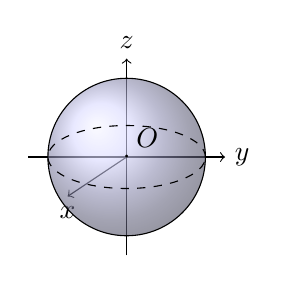
\begin{tikzpicture}[scale=0.5, baseline=(current bounding box.center)]
            \draw[->] (-2.5,0) -- (2.5,0) node[right] {$y$};
            \draw[->] (0,-2.5) -- (0,2.5) node[above] {$z$};
            \draw[->] (0,0) -- (-1.5,-1) node[below] {$x$};
            \shade[ball color=blue!20, opacity=0.6] (0,0) circle (2cm);
            \draw (0,0) circle (2cm);
            \draw[dashed] (0,0) ellipse (2cm and 0.8cm);
            \node at (0,0) {$\cdot$};
            \node[above right] at (0,0) {$O$};
        \end{tikzpicture} & 
        $(x-x_0)^2 + (y-y_0)^2 + (z-z_0)^2 = R^2$ \\
        \hline
        椭球面 & 
        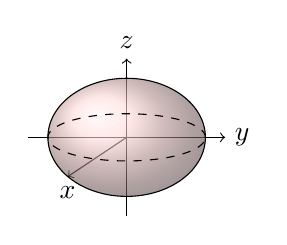
\begin{tikzpicture}[scale=0.5, baseline=(current bounding box.center)]
            \draw[->] (-2.5,0) -- (2.5,0) node[right] {$y$};
            \draw[->] (0,-2) -- (0,2) node[above] {$z$};
            \draw[->] (0,0) -- (-1.5,-1) node[below] {$x$};
            \shade[ball color=red!20, opacity=0.6] (0,0) ellipse (2cm and 1.5cm);
            \draw (0,0) ellipse (2cm and 1.5cm);
            \draw[dashed] (0,0) ellipse (2cm and 0.6cm);
        \end{tikzpicture} & 
        $\dfrac{x^2}{a^2} + \dfrac{y^2}{b^2} + \dfrac{z^2}{c^2} = 1$ \\
        \hline
        圆柱面 & 
        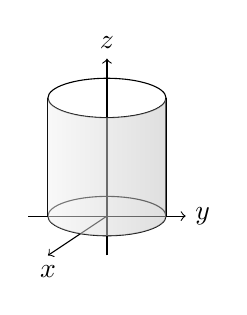
\begin{tikzpicture}[scale=0.5, baseline=(current bounding box.center)]
            \draw[->] (-2,0) -- (2,0) node[right] {$y$};
            \draw[->] (0,-1) -- (0,4) node[above] {$z$};
            \draw[->] (0,0) -- (-1.5,-1) node[below] {$x$};
            \draw (0,3) ellipse (1.5cm and 0.5cm);
            \draw (0,0) ellipse (1.5cm and 0.5cm);
            \draw (-1.5,3) -- (-1.5,0);
            \draw (1.5,3) -- (1.5,0);
            \shade[left color=gray!10, right color=gray!50, opacity=0.5] (-1.5,0) arc (180:360:1.5cm and 0.5cm) -- (1.5,3) arc (0:-180:1.5cm and 0.5cm) -- cycle;
        \end{tikzpicture} & 
        \begin{tabular}{@{}c@{}}$x^2 + y^2 = R^2$\\(母线平行于 $z$ 轴)\end{tabular} \\
        \hline
    \end{tabular}
\end{table}

\begin{table}[htbp]
    \centering
    \caption{常见空间曲面 II}
    \begin{tabular}{|c|c|c|}
        \hline
        \textbf{曲面名称} & \textbf{图形} & \textbf{方程} \\
        \hline
        圆锥面 & 
        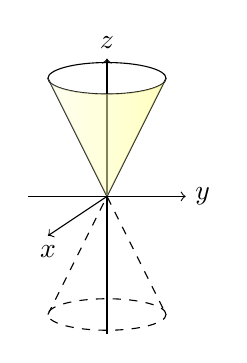
\begin{tikzpicture}[scale=0.5, baseline=(current bounding box.center)]
            \draw[->] (-2,0) -- (2,0) node[right] {$y$};
            \draw[->] (0,-3.5) -- (0,3.5) node[above] {$z$};
            \draw[->] (0,0) -- (-1.5,-1) node[below] {$x$};
            \draw (0,3) ellipse (1.5cm and 0.4cm);
            \draw (-1.5,3) -- (0,0) -- (1.5,3);
            \shade[left color=yellow!10, right color=yellow!50, opacity=0.5] (0,0) -- (1.5,3) arc (0:-180:1.5cm and 0.4cm) -- cycle;
            \draw[dashed] (0,-3) ellipse (1.5cm and 0.4cm);
            \draw[dashed] (-1.5,-3) -- (0,0) -- (1.5,-3);
        \end{tikzpicture} & 
        \begin{tabular}{@{}c@{}}$z^2 = a^2(x^2 + y^2)$ \\ (顶点在原点)\end{tabular} \\
        \hline
        旋转抛物面 & 
        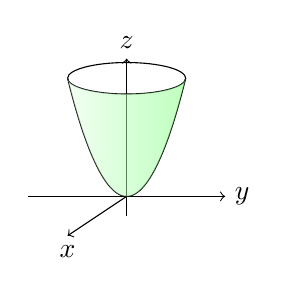
\begin{tikzpicture}[scale=0.5, baseline=(current bounding box.center)]
            \draw[->] (-2.5,0) -- (2.5,0) node[right] {$y$};
            \draw[->] (0,-0.5) -- (0,3.5) node[above] {$z$};
            \draw[->] (0,0) -- (-1.5,-1) node[below] {$x$};
            \draw (0,3) ellipse (1.5cm and 0.4cm);
            \draw (-1.5,3) parabola bend (0,0) (1.5,3);
            \shade[left color=green!10, right color=green!50, opacity=0.5] (-1.5,3) parabola bend (0,0) (1.5,3) arc (0:-180:1.5cm and 0.4cm);
        \end{tikzpicture} & 
        $z = a(x^2 + y^2)$ \\
        \hline
        \begin{tabular}{@{}c@{}}双曲抛物面\\(马鞍面)\end{tabular} & 
        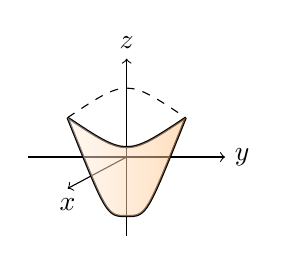
\begin{tikzpicture}[scale=0.5, baseline=(current bounding box.center)]
            \draw[->] (-2.5,0) -- (2.5,0) node[right] {$y$};
            \draw[->] (0,-2) -- (0,2.5) node[above] {$z$};
            \draw[->] (0,0) -- (-1.5,-0.8) node[below] {$x$};
            \draw[thick] (-1.5,1) .. controls (0,0) .. (1.5,1);
            \draw[thick] (-1.5,1) .. controls (-0.5,-1.5) .. (0,-1.5);
            \draw[thick] (1.5,1) .. controls (0.5,-1.5) .. (0,-1.5);
            \draw[dashed] (-1.5,1) .. controls (0,2) .. (1.5,1);
            \shade[left color=orange!10, right color=orange!50, opacity=0.5] (-1.5,1) .. controls (0,0) .. (1.5,1) .. controls (0.5,-1.5) .. (0,-1.5) .. controls (-0.5,-1.5) .. (-1.5,1);
        \end{tikzpicture} & 
        $z = \dfrac{x^2}{a^2} - \dfrac{y^2}{b^2}$ \\
        \hline
        单叶双曲面 & 
        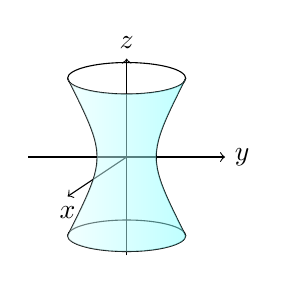
\begin{tikzpicture}[scale=0.5, baseline=(current bounding box.center)]
            \draw[->] (-2.5,0) -- (2.5,0) node[right] {$y$};
            \draw[->] (0,-2.5) -- (0,2.5) node[above] {$z$};
            \draw[->] (0,0) -- (-1.5,-1) node[below] {$x$};
            \draw (0,2) ellipse (1.5cm and 0.4cm);
            \draw (0,-2) ellipse (1.5cm and 0.4cm);
            \draw (-1.5,2) .. controls (-0.5,0) .. (-1.5,-2);
            \draw (1.5,2) .. controls (0.5,0) .. (1.5,-2);
            \shade[left color=cyan!10, right color=cyan!50, opacity=0.5] (-1.5,2) .. controls (-0.5,0) .. (-1.5,-2) arc (180:360:1.5cm and 0.4cm) .. controls (0.5,0) .. (1.5,2) arc (0:-180:1.5cm and 0.4cm);
        \end{tikzpicture} & 
        \begin{tabular}{@{}c@{}}$\dfrac{x^2}{a^2} + \dfrac{y^2}{b^2} - \dfrac{z^2}{c^2} = 1$ \\ ($z$ 轴为中心轴) \end{tabular} \\
        \hline
        双叶双曲面 & 
        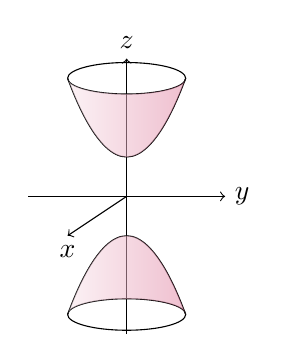
\begin{tikzpicture}[scale=0.5, baseline=(current bounding box.center)]
            \draw[->] (-2.5,0) -- (2.5,0) node[right] {$y$};
            \draw[->] (0,-3.5) -- (0,3.5) node[above] {$z$};
            \draw[->] (0,0) -- (-1.5,-1) node[below] {$x$};
            % Upper sheet
            \draw (-1.5,3) parabola bend (0,1) (1.5,3);
            \draw (0,3) ellipse (1.5cm and 0.4cm);
            \shade[left color=purple!10, right color=purple!50, opacity=0.5] (-1.5,3) parabola bend (0,1) (1.5,3) arc (0:-180:1.5cm and 0.4cm);
            % Lower sheet
            \draw (-1.5,-3) parabola bend (0,-1) (1.5,-3);
            \draw (0,-3) ellipse (1.5cm and 0.4cm);
            \shade[left color=purple!10, right color=purple!50, opacity=0.5] (-1.5,-3) parabola bend (0,-1) (1.5,-3) arc (0:180:1.5cm and 0.4cm);
        \end{tikzpicture} & 
        \begin{tabular}{@{}c@{}}$\dfrac{x^2}{a^2} + \dfrac{y^2}{b^2} - \dfrac{z^2}{c^2} = -1$ \\ (即 $\dfrac{z^2}{c^2} - \dfrac{x^2}{a^2} - \dfrac{y^2}{b^2} = 1$) \end{tabular} \\
        \hline
    \end{tabular}
\end{table}

\subsection{旋转曲面}
\begin{theorem}[任意曲线绕任意轴旋转的曲面方程]
    设空间曲线 $\Gamma: \begin{cases} F(x, y, z) = 0 \\ G(x, y, z) = 0 \end{cases}$．
    旋转轴 $L$ 过点 $M_0(x_0, y_0, z_0)$，方向向量为 $\boldsymbol{s} = (m, n, p)$．

    设 $P(x, y, z)$ 为旋转曲面上任一点，则它是由曲线 $\Gamma$ 上的某点 $P_1(x_1, y_1, z_1)$ 绕轴 $L$ 旋转得到的．点 $P$ 的坐标 $(x, y, z)$ 必须满足以下条件：
    \begin{enumerate}
        \item 点 $P$ 和 $P_1$ 到定点 $M_0$ 的距离相等（位于以 $M_0$ 为球心的球面上）：
        \[ (x-x_0)^2 + (y-y_0)^2 + (z-z_0)^2 = (x_1-x_0)^2 + (y_1-y_0)^2 + (z_1-z_0)^2 \]
        \item 向量 $\overrightarrow{M_0P}$ 和 $\overrightarrow{M_0P_1}$ 在轴方向 $\boldsymbol{s}$ 上的投影相等（位于同一垂直于轴的平面上）：
        \[ m(x-x_0) + n(y-y_0) + p(z-z_0) = m(x_1-x_0) + n(y_1-y_0) + p(z_1-z_0) \]
    \end{enumerate}
    将曲线方程 $\begin{cases} F(x_1, y_1, z_1) = 0 \\ G(x_1, y_1, z_1) = 0 \end{cases}$ 与上述两式联立，消去 $x_1, y_1, z_1$，得到的关于 $x, y, z$ 的方程即为旋转曲面方程．
\end{theorem}

\begin{itemize}
    \item \textbf{特例 1}：若曲线 $C:\begin{cases} f(y,z)=0 \\ x=0 \end{cases}$ 绕 $z$ 轴旋转，得到的方程为 $f(\pm\sqrt{x^2+y^2}, z) = 0$．
    \item \textbf{特例 2}：若曲线 $C:\begin{cases} f(x,y)=0 \\ z=0 \end{cases}$ 绕 $x$ 轴旋转，得到的方程为 $f(x, \pm\sqrt{y^2+z^2}) = 0$．
\end{itemize}

\begin{corollary}[直线绕坐标轴旋转]
    设直线 $L$ 的参数方程为 $\begin{cases} x = x_0 + mt \\ y = y_0 + nt \\ z = z_0 + pt \end{cases}$．
    若该直线绕 $z$ 轴旋转，则旋转曲面的参数方程为
    \[
        \begin{cases}
            x = \sqrt{(x_0+mt)^2 + (y_0+nt)^2} \cos\theta \\
            y = \sqrt{(x_0+mt)^2 + (y_0+nt)^2} \sin\theta \\
            z = z_0 + pt
        \end{cases} \quad (0 \le \theta < 2\pi, t \in \mathbb{R})
    \]
    消去参数 $t, \theta$ 即可得到隐函数方程：
    \[
        x^2 + y^2 = \left(x_0 + m\frac{z-z_0}{p}\right)^2 + \left(y_0 + n\frac{z-z_0}{p}\right)^2 \quad (\text{当 } p \ne 0)
    \]
    同理可得绕 $x$ 轴或 $y$ 轴旋转的参数方程．
\end{corollary}

\begin{example}
    求直线 $\begin{cases}
        x = 3 - t\\
        y = -1 + t\\
        z = 1 + 2t
        \end{cases}$ 绕 $y$ 轴旋转一周所成曲面的方程．
\end{example}
\begin{solution}
    设直线上任意一点为 $P_1(x_1, y_1, z_1)$，则有
    \[
        \begin{cases}
            x_1 = 3 - t\\
            y_1 = -1 + t\\
            z_1 = 1 + 2t
        \end{cases}
    \]
    由第二式得 $t = y_1 + 1$．代入另两式，消去参数 $t$，得到 $x_1, z_1$ 与 $y_1$ 的关系：
    \[
        \begin{cases}
            x_1 = 3 - (y_1 + 1) = 2 - y_1 \\
            z_1 = 1 + 2(y_1 + 1) = 2y_1 + 3
        \end{cases}
    \]
    该点绕 $y$ 轴旋转一周，其旋转轨迹上的任意一点 $P(x,y,z)$ 满足：
    \begin{enumerate}
        \item 高度不变：$y = y_1$
        \item 到旋转轴（$y$轴）的距离相等：$x^2 + z^2 = x_1^2 + z_1^2$
    \end{enumerate}
    将 $x_1, z_1$ 用 $y$ 表示（因为 $y_1=y$）代入距离公式：
    \[
        x^2 + z^2 = (2 - y)^2 + (2y + 3)^2
    \]
    整理得：
    \[
        x^2 + z^2 = 4 - 4y + y^2 + 4y^2 + 12y + 9
    \]
    即曲面方程为：
    \[
        x^2 - 5y^2 + z^2 - 8y - 13 = 0
    \]
\end{solution}

\section{多元函数微分在空间几何的应用}
\subsection{曲线的切线和法平面}
\begin{theorem}
    设空间曲线 $\Gamma$ 的参数方程为 $\begin{cases} x = x(t) \\ y = y(t) \\ z = z(t) \end{cases}$，那么在$t=t_0$处的切向量为
    \[\left( x'(t_0), y'(t_0), z'(t_0) \right)\]
    若在 $t=t_0$ 处满足 $x'(t_0)^2 + y'(t_0)^2 + z'(t_0)^2 \ne 0$．
    则曲线 $\Gamma$ 在点 $P(x(t_0), y(t_0), z(t_0))$ 处的切线方程为
    \[
        \frac{x - x(t_0)}{x'(t_0)} = \frac{y - y(t_0)}{y'(t_0)} = \frac{z - z(t_0)}{z'(t_0)}
    \]
    法平面方程为
    \[
        x'(t_0)(x - x(t_0)) + y'(t_0)(y - y(t_0)) + z'(t_0)(z - z(t_0)) = 0
    \]
\end{theorem}

\begin{example}
    求曲线 $\begin{cases}
        x = y^2\\
        z = x^2
    \end{cases}$ 在点 $(1,1,1)$ 处的切线与法平面．
\end{example}
\begin{solution}
    容易得到参数方程为
    \[ \begin{cases} x=t^2 \\ y=t \\ z=t^4 \end{cases} \]

    对参数$t$求导，得到切线向量：
    \[ \frac{dx}{dt} = 2t, \quad \frac{dy}{dt} = 1, \quad \frac{dz}{dt} = 4t^3 \]
    
    在点$(1,1,1)$处，$t=1$，切线向量为
    \[ \bm{n} = (2, 1, 4) \]
    
    因此，切线方程为
    \[ \frac{x-1}{2} = \frac{y-1}{1} = \frac{z-1}{4} \]
    
    在曲线中，切向量$\bm{n}$即为法平面的法向量，因此，

    法平面方程为
    \[ 2(x-1) + 1(y-1) + 4(z-1) = 0 \]
    
\end{solution}

\begin{example}
    求曲线 $\begin{cases}
        x^2 + y^2 + z^2 -3x =0\\
        2x - 3y + 5z - 4 = 0
    \end{cases}$ 在点 $(1,1,1)$ 处的切线与法平面方程．
\end{example}
\begin{solution}
    注意到曲线 $\Gamma$ 是两个曲面 $\Sigma_1: x^2 + y^2 + z^2 -3x =0$ 和 $\Sigma_2: 2x - 3y + 5z - 4 = 0$ 的交线．\\
    则曲线上任意一点的切向量都与两个平面的法向量垂直．因此，切向量 $\bm{n}$ 可以通过两个平面的法向量的叉积得到．\\
    $\Sigma_1$ 的法向量为 $\nabla F = (2x - 3, 2y, 2z)$，$\Sigma_2$ 的法向量为 $\nabla G = (2, -3, 5)$．
    在点 $(1,1,1)$ 处，$\nabla F = (-1, 2, 2)$，$\nabla G = (2, -3, 5)$．
    则切向量为
    \[ \bm{n} = \nabla F \times \nabla G = (16, -9, -1) \]
    因此，切线方程为
    \[ \frac{x-1}{16} = \frac{y-1}{-9} = \frac{z-1}{-1} \]
    法平面方程为
    \[ 16(x-1) - 9(y-1) - (z-1) = 0 \]

\end{solution}
\subsection{曲面的法线和切平面}
\begin{theorem}
    设空间曲面 $\Sigma$ 的隐函数方程为 $F(x, y, z) = 0$，则在点$P(x_0, y_0, z_0)$处的法向量为
    \[ \left( F_x(x_0, y_0, z_0), F_y(x_0, y_0, z_0), F_z(x_0, y_0, z_0) \right) \]
    若在点 $P$ 处满足 $F_x^2 + F_y^2 + F_z^2 \ne 0$．
    则曲面 $\Sigma$ 在点 $P$ 处的法线方程为
    \[
        \frac{x - x_0}{F_x} = \frac{y - y_0}{F_y} = \frac{z - z_0}{F_z}
    \]
    切平面方程为
    \[
        F_x(x - x_0) + F_y(y - y_0) + F_z(z - z_0) = 0
    \]
\end{theorem}



\ifx\allfiles\undefined
\end{document}
\fi